\subsection{The Workflow tab}
\label{sec:workflow_tab}

This tab gives information about the workflow, that can be accessed by clicking on the available sub-tabs:

\begin{itemize}
\item {\bf Task dependencies}. It shows the connection between each task
  and sub-workflows. The tasks are the individual processing steps
  that run a specific pipeline recipe. A sub-workflow groups tasks
  of similar purposes to simplify the overall data flow structure.
  Each sub-workflow is also illustrated with the relations between the
  tasks within it.

  The tasks descriptor indicates the name of the task, the recipe,
  the main input and the associated inputs. The descriptor also
  indicates whether an associated input has to satisfy a certain
  condition to be associated (e.g., a calibration X is associated only
  if the user specifies it in the preferences, or if the main input is
  obtained with a certain instrument setup). Descriptor for the
  sub-workflows indicates the tasks within it, and the corresponding
  main inputs and recipes.

  The colour of the lines connecting tasks and sub-workflows mirror the
  colour they have inside the descriptors. Figure \ref{fig:workflow_tab} shows an example of this tab.

\begin{figure}[h!]
\centering
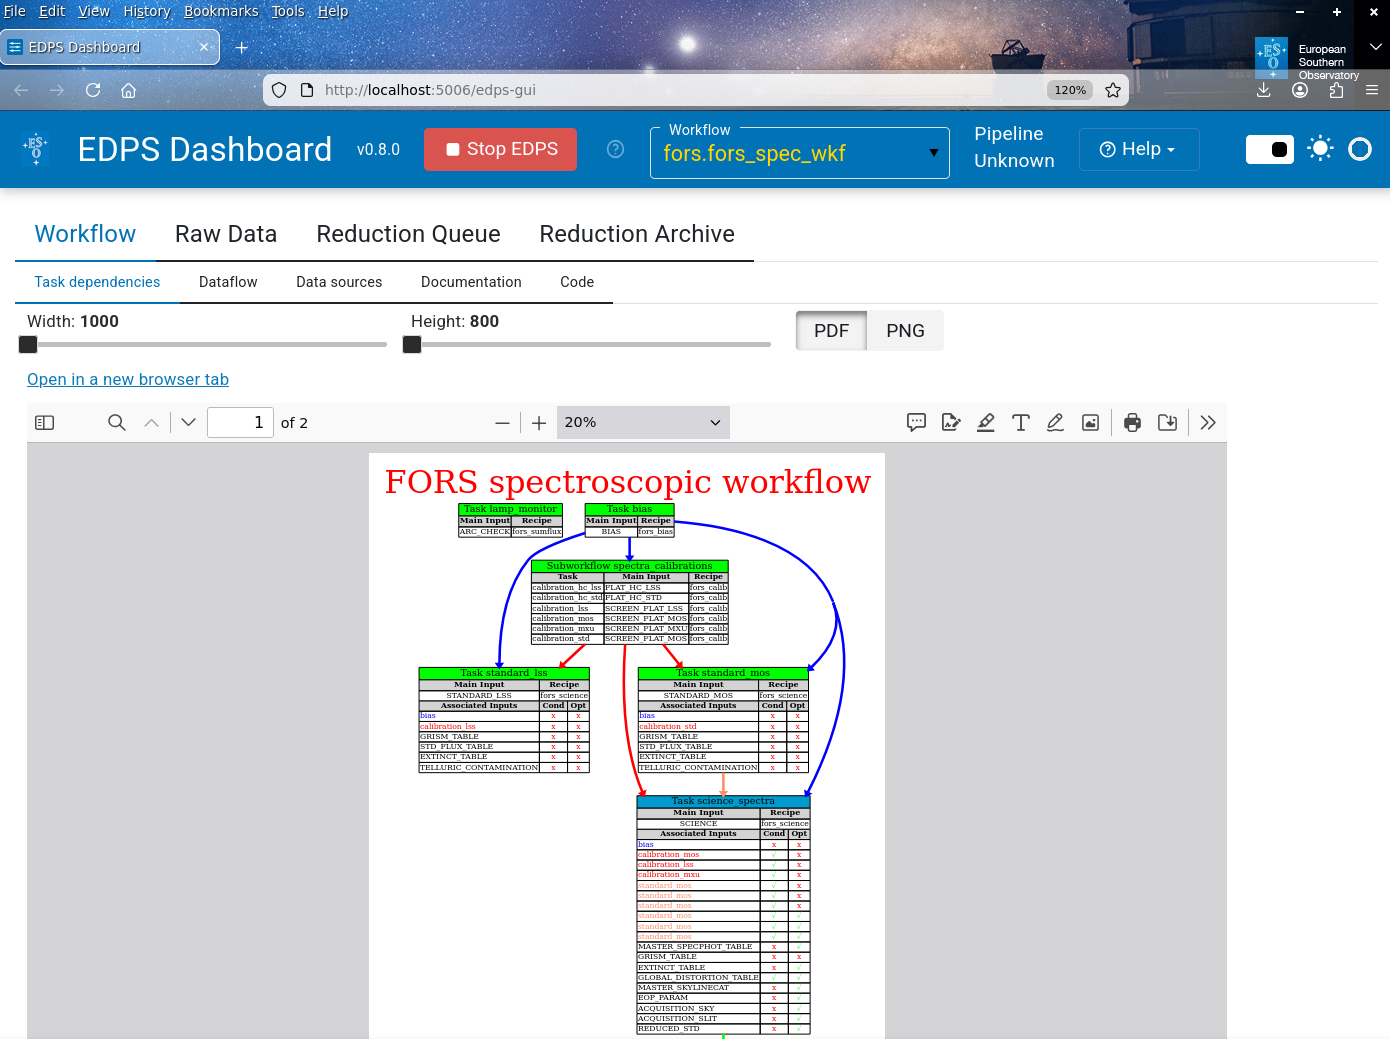
\includegraphics[width=0.9\textwidth]{figures/workflow-tab.jpg}
\caption{The \edps\ dashboard, showing part of the task dependencies within the FORS2 spectroscopic workflow.}
\label{fig:workflow_tab}
\end{figure}


\item {\bf Dataflow}. It is a simpler representation of the workflow. It
  shows the categories of the data sources of the raw data, the
  individual tasks (in green) and the sub-workflows (in orange). It
  provides a global view of the data reduction chain. Figure \ref{fig:load_flow} shows an example of this tab.


\begin{figure}[h!]
\centering
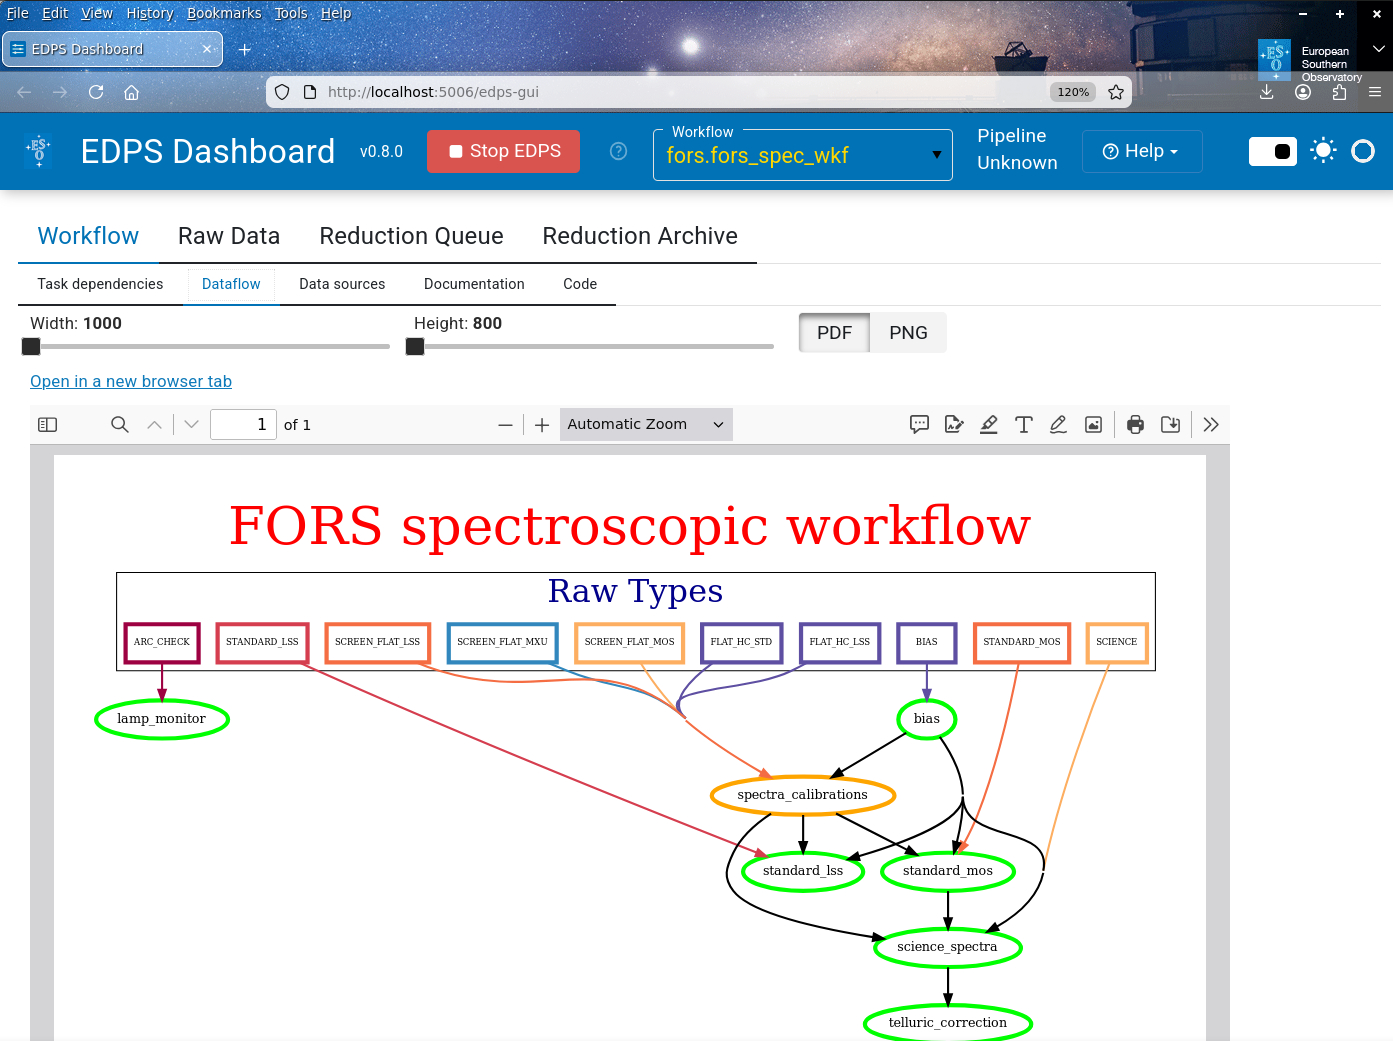
\includegraphics[width=0.9\textwidth]{figures/load-flow.jpg}
\caption{The \edps\ dashboard, showing the top-level data flow structure of the FORS2 spectroscopic workflow.}
\label{fig:load_flow}
\end{figure}


\item {\bf Data sources}. It shows the association map, with the definition of the various data-sources, their properties
  such as

\begin{itemize}
    \item {\bf Classification}. The types of files that belong to this
      data-source. The classification is the tag assigned to the file
      used by the processing recipe. Note that a single data-source
      (e.g. SCIENCE) can include files with different classifications
      (e.g., SCIENCE\_LSS, SCIENCE\_MOS, SCIENCE\_MXU), as they are
      processed by different algorithms by the pipeline recipe (fors\_science).

    \item {\bf setup}. The list of header keywords used to recognize the
      instrumental setup used to obtain those observations.

    \item {\bf grouping}. The list of header keywords used to group the files
      within the same classification. Files of the same group (e.g. that
      have the same value of the header keywords in this list) are input
      to the same recipe execution.

    \item {\bf Task}. The name of the task that have that data-source as main
      input. Note that a data-source can be the main input of more than
      one task.

    \item {\bf Recipe}. The name of the recipe executed to process that
      data-source. Because a data-source can be the main input of more
      than one task, it can be processed by more than one recipe.

    \item {\bf Static calibrations}. Association map between static
      calibrations, data-sources, and tasks. An `x` indicates that that
      static calibration is needed by a given task to process a given
      data-source.
\end{itemize}

\item {\bf Documentation}. Links to the relevant documentation files for
  that pipeline.

\item {\bf Code}. It shows the Python code of each file in the
  workflow. The drop-down menu `Select file` allows to select the
  file to inspect. Files cannot be edited from the GUI. If changes are needed, edit the file with an external editor, 
  close and reopen the EDP-GUI for the modification to have an effect.

  \end{itemize}